\documentclass[sigconf]{acmart}
\setcounter{secnumdepth}{3}
\usepackage{graphicx}
\usepackage[export]{adjustbox}
\settopmatter{printfolios=true}
%% \BibTeX command to typeset BibTeX logo in the docs
\AtBeginDocument{%
  \providecommand\BibTeX{{%
    \normalfont B\kern-0.5em{\scshape i\kern-0.25em b}\kern-0.8em\TeX}}}

%% Rights management information.  This information is sent to you
%% when you complete the rights form.  These commands have SAMPLE
%% values in them; it is your responsibility as an author to replace
%% the commands and values with those provided to you when you
%% complete the rights form.
\copyrightyear{2019}
\acmYear{2019}
\setcopyright{rightsretained}

%%
%% Submission ID.
%% Use this when submitting an article to a sponsored event. You'll
%% receive a unique submission ID from the organizers
%% of the event, and this ID should be used as the parameter to this command.
%%\acmSubmissionID{123-A56-BU3}

%%
%% end of the preamble, start of the body of the document source.
\begin{document}

\title{Heimdall: USB mass storage devices analysis using network isolated embeded device}

%%
%% The "author" command and its associated commands are used to define
%% the authors and their affiliations.
%% Of note is the shared affiliation of the first two authors, and the
%% "authornote" and "authornotemark" commands
%% used to denote shared contribution to the research.
\author{Ivan Zlatanov}
\affiliation{%
  \role{Author}\\
  \institution{National Trade and Banking High School}
  \country{Sofia, Bulgaria}
}
\email{ivanff123@gmail.com}

\author{Yavor Papazov}
\affiliation{%
  \role{Mentor}\\
  \institution{European Software Institute - Center Eastern Europe}
  \country{Sofia, Bulgaria}
}
\email{yavorpap@gmail.com}

\renewcommand{\shortauthors}{Ivan and Yavor}

\begin{abstract}
\quad One of the most frequently used serial communication protocol on almost any modern computer-like device is the Universal Serial Bus (USB). It allows connecting storage devices and other peripheral devices to a computer. USB storage devices are frequently used for cyberattack, malware distribution and data theft on different systems. Some antivirus softwares provide USB scans but they are limited to malware detection. Because of that USB storage devices are banned or limited in major companies and government agencies around the world. In this paper we propose a network isolated embedded system that performs tests designed to detect different kind of exploits and malicious behaviour that are left undetected by almost any antivirus software.
\end{abstract}

%%
%% Keywords. The author(s) should pick words that accurately describe
%% the work being presented. Separate the keywords with commas.
\keywords{universal serial bus, usb vulnerabilities, firmware exploitation, cybersecurity}

\maketitle

\section{Introduction}
\par \quad The Universal Serial Bus (USB) is one of the most widely used and successful serial communication standards which is enforced in almost any computer today. The main idea behind this standard is to provide interface for multiple external devices connected to one host.

\par Despite the popularity of the Universal Serial Bus, devices like USB flash drives are restricted or fully banned in the enterprise world because of the security risks they pose. During the early days of computers, the most common way to transfer files from one device to another was through a diskette. However, this method proved to be inefficient when it comes to security due to its usage for computer virus distribution on different devices. Today floppy disks still exist but their storage capacity is not nearly enough compared to their successor - the USB mass storage device. This renders diskettes useless in practice this days.

\par It was known that a USB mass storage device can be used to infect different kinds of computer-like systems, steal data or compromise their integrity. Security threats like Stuxnet\cite{stuxnet} and Flame\cite{flame} proved that a system with vulnerability that can be exploited via a USB flash drive combined with a human factor may cause catastrophic failures with high financial damages.

\par In this paper, we propose a network isolated embedded system that is able to perform a stack of specific tests in order to identify potential malicious intent and/or malfunction in a USB storage device. The USB is inspected, sealed and analyzed by emulating different environments, situations and user interactions. All of the used methods aim to find different exploits - file infection by the firmware, data corruption, malware infection, automatic code execution, electrical attacks by USB killers and etc.

\section{Related Work}
\par \quad In this section, we discuss work related to USB security and vulnerabilities. We also explain why some methods in these works seem efficient in most cases but are not applicable in real targeted attacks. These research papers concentrate on user authentication bypassing.
\par Secure USB bypassing tool \cite{secure_usb_bps} by Jewan Bang, Byeongyeong Yoo and Sangjin Lee studies secure USB functions, how to bypass them with USB controller commands in order to retrieve data and the implementation of a secure USB bypassing tool. The paper explores in details how USB security functions work and the possible vulnerabilities they have.
\par Most of the researches in the field analyze the security vulnerabilities or present methods for malware detection that are designed to work on the host's computer. Although these methods are efficient, they do not guarantee that the machine performing them will not get infected and spread the virus through the network or get its hardware damaged from a power shock. Even if the host system has its network adapter programmatically disabled, it can still be activated by an undetected rootkit.

\section{Background}
\par \quad In this section, we discuss various attacks, performed by or with the help of a USB. We also discuss an attack called "Drop attack" and why it is so important.

\subsection{Attacks}
\subsubsection{Firmware exploitation}
\par \quad The firmware of almost any USB mass storage device can be alternated using multiple leaked OEM tools like Patriot. By modifying this software an attacker can accomplish different goals - changing information about the vendor and the model of the device, creating procedures which can infect files during the transfer between the host and the USB, creating backdoors into systems or mimicking input or output devices.

\subsubsection{Power Surge}
\par \quad The power surge attack is executed using usb-like device that collects electricity from its host, passes it through high-voltage generators that increase its current and voltage and charges it into capacitors. Once the capacitors are full the device discharges them into the host's port. The process keeps repeating until the port is damaged and cannot supply the USB with electricity anymore. The aim of this attack is to damage hardware components. A USB killer device can be bought for around fifty dollars from popular online retailers. Although it seems useless, such a device has been used to destroy hundreds of computers resulting in thousands of dollars in damages. 
Figure \ref{fig:usb_killer_diagram} is a simple illustration of the process.

 \begin{figure}[htp]
    \centering
    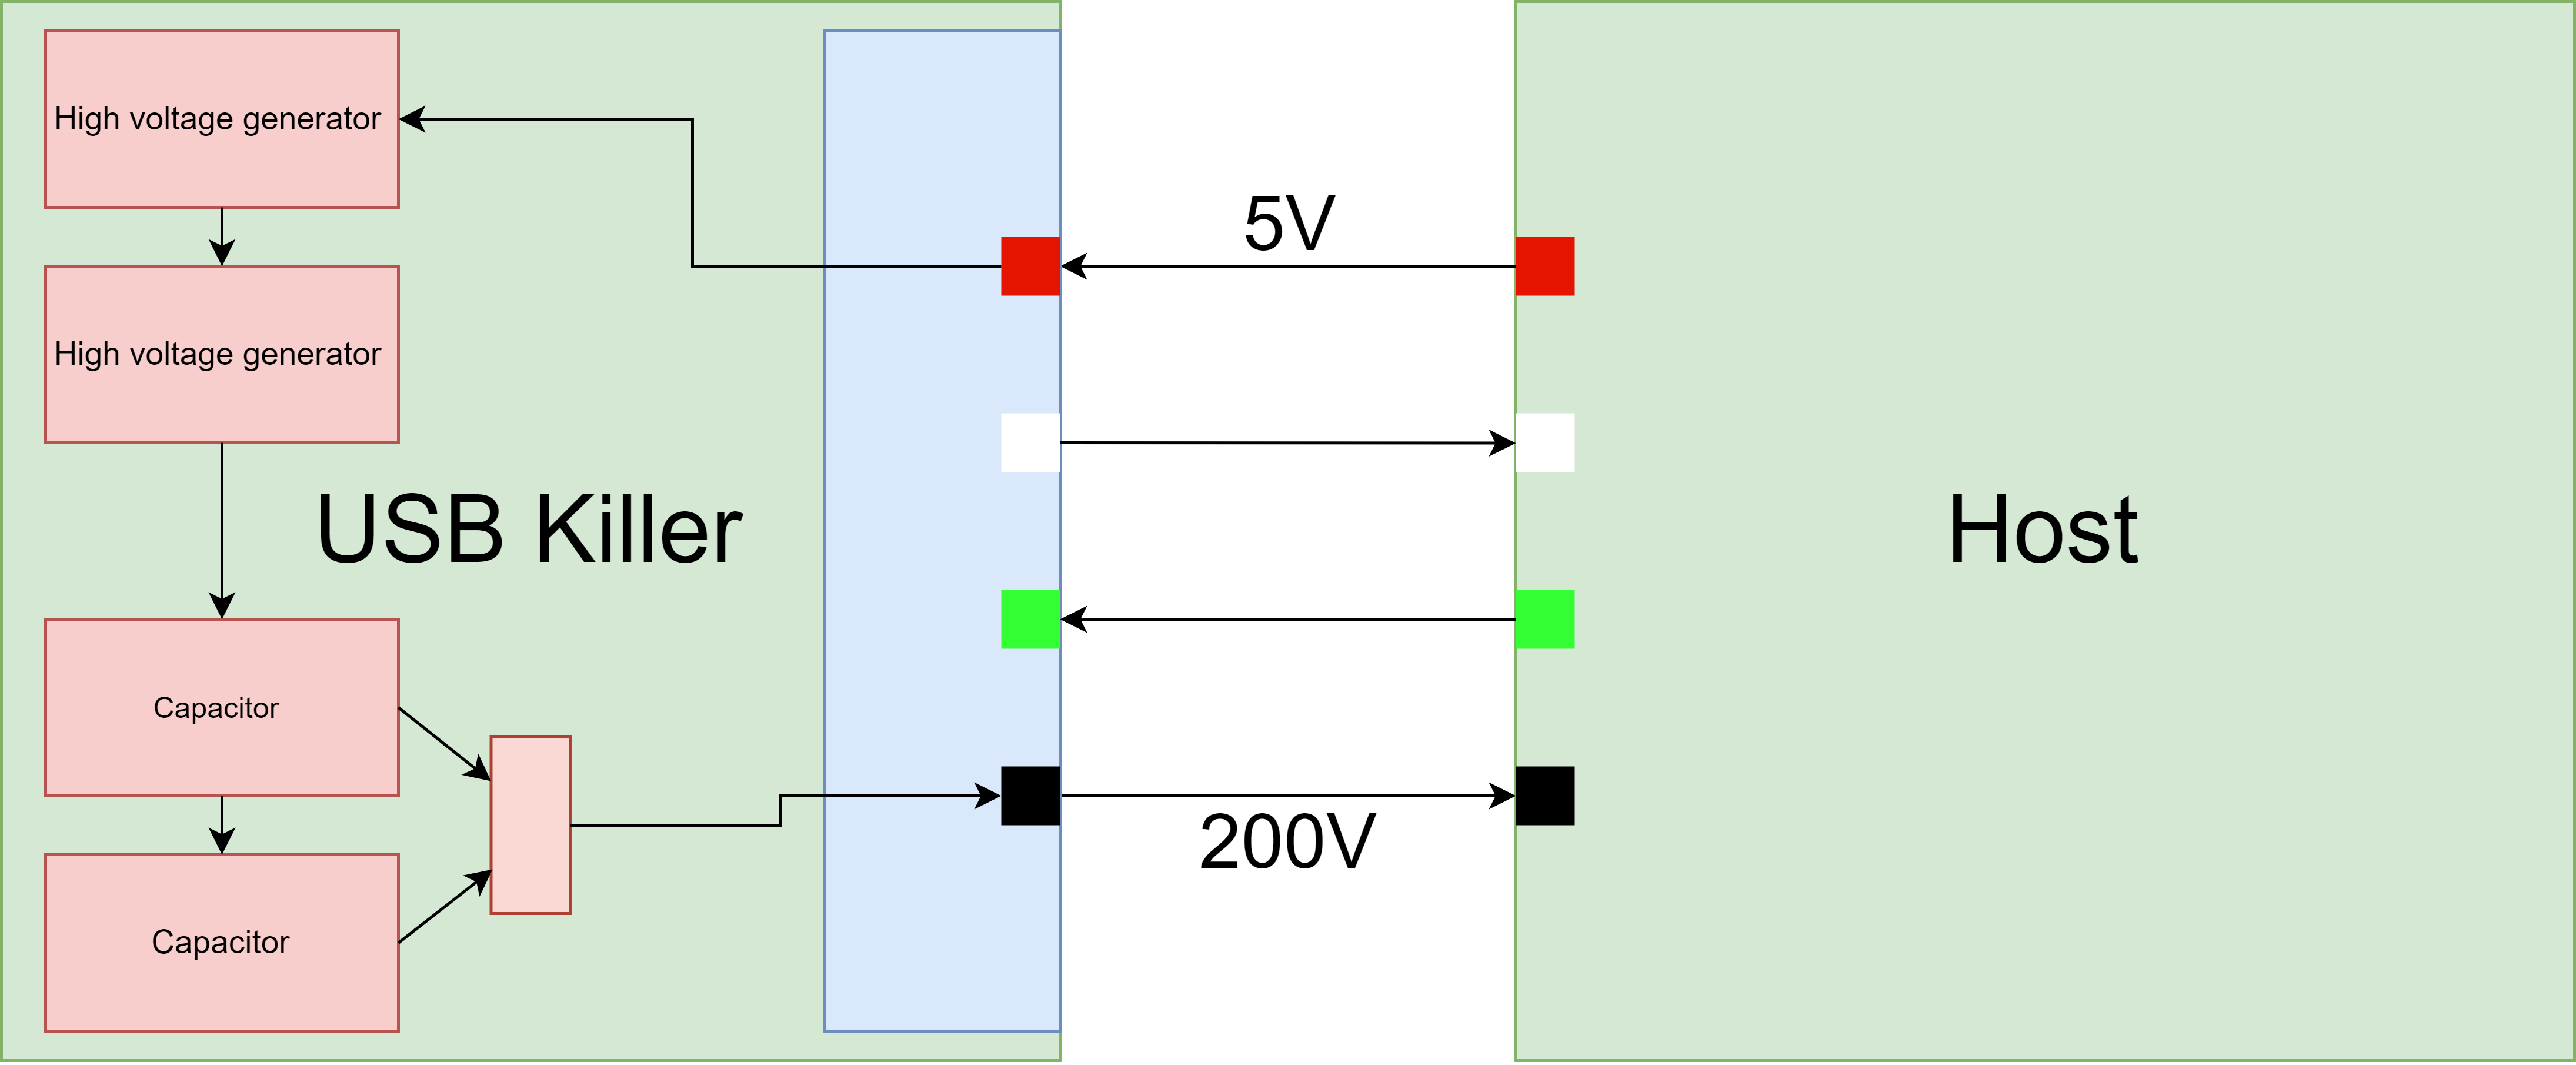
\includegraphics[width=\linewidth]{images/usb_killer_diagram.png}
    \caption{The diagram shows how USB killer works in a simplified way.}
    \label{fig:usb_killer_diagram}
\end{figure}

\subsubsection{USBee}
\par \quad Network isolated systems \cite{usbee} present in almost any complex of importance. Because malfunctions of these facilities can lead to catastrophic failures, the computers systems inside have to be cut off from the outside world in order to eliminate the risk of an attack through the internet. USBee is designed to infiltrate and infect such systems with a specially designed malware that finds a connected USB device and, when the attacker wants it, to send a sequence of zeros. That action causes the device to vibrate and produce sound at detectable frequencies between 240 and 480Mhz. The sound can be detected via receiver nearby the USB. Although the transmission rate is low it is still efficient for obtaining confidential information.

\subsubsection{Malicious Boot Rerouting}
\par \quad USB storage device with a specifically modified firmware can function as a hijacking boot device during the bootloading process of its host. The host will boot from the USB which will load a malicious content - usually malware or a rootkit. Then the boot process will continue with booting the real OS. Figure \ref{fig:bootloading_rerouting} illustrates the rerouting of the bootloading process. 

\begin{figure}[htp]
    \centering
    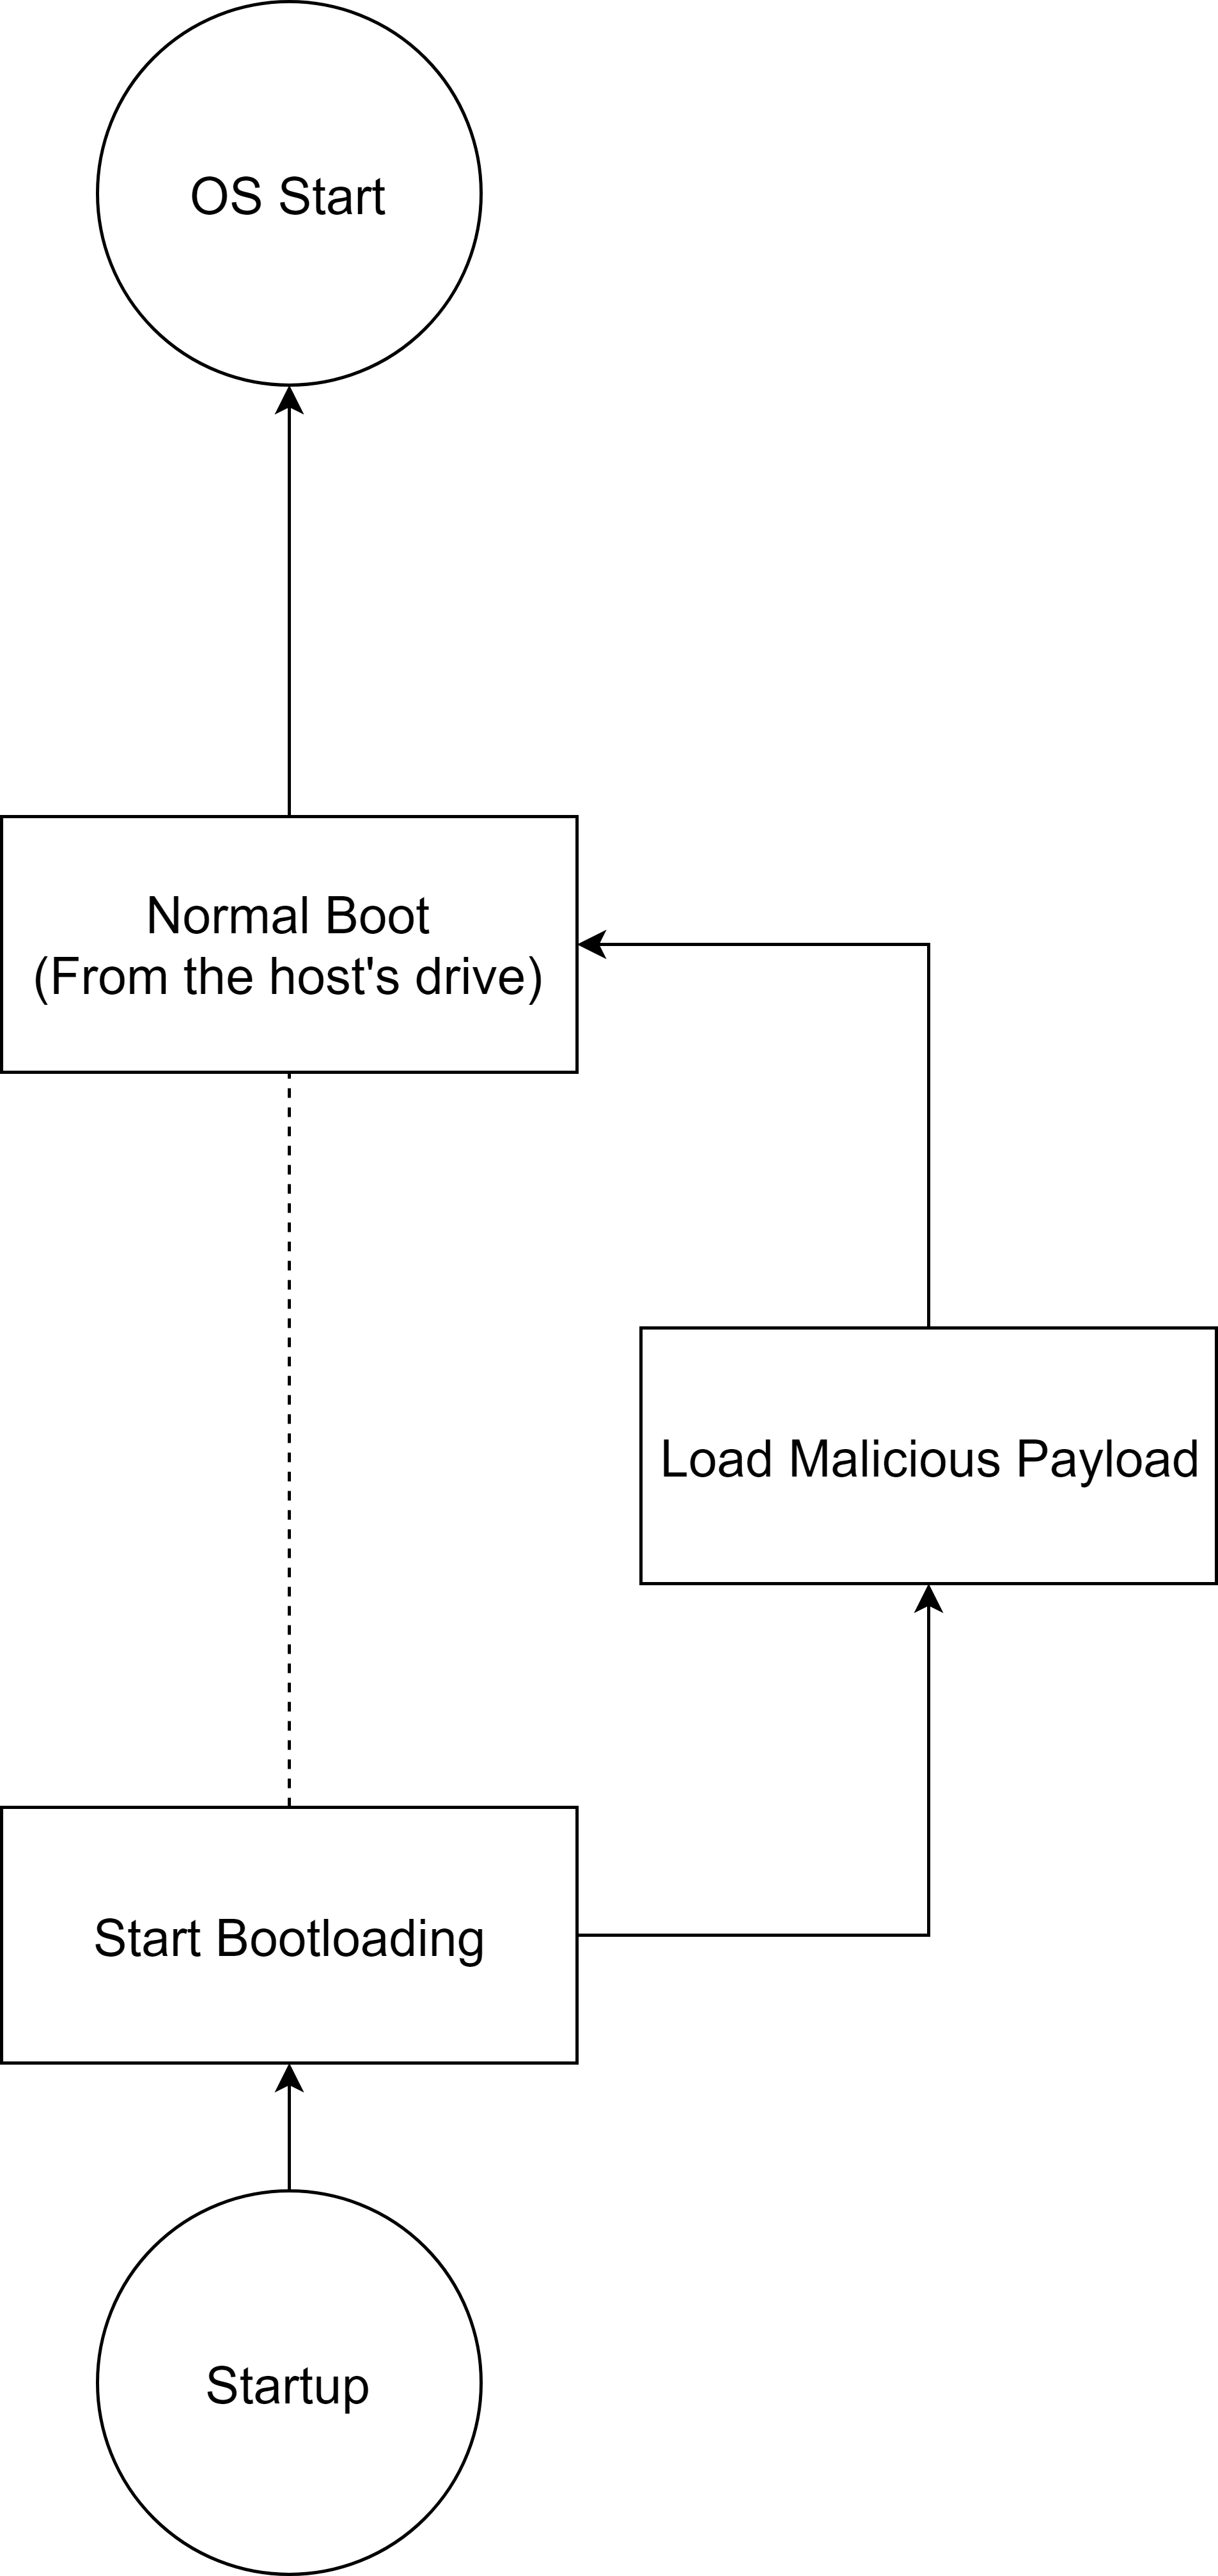
\includegraphics[width=\linewidth]{images/bootloading_rerouting.png}
    \caption{The diagram shows in a simplified way how a USB malicious boot rerouting works.}
    \label{fig:bootloading_rerouting}
\end{figure}

\subsection{How USBs spread malware}
\subsubsection{What is a "USB drop attack"}
\par \quad Hackers used to place programmatically alternated USB drives in strategical location for years. The main idea behind this practice is that somebody will find and use it. The attack relies on social engineering in which case the attacker tricks a victim into plugging the USB storage device into his computer device. Social engineering can be further used to trick the victim into opening files or links on the USB and possibly infecting his the machine.
\par The USBs are usually placed in public locations - parking lots, hallways, classrooms or common rooms. This way the chances of a drive getting picked up and used increases.

\subsubsection{Attack effectiveness}
\par \quad The attack leverages humans' inner curiosity \cite{usb_drop_attack} and uses it against them. Once a device is taken the chances that it will be used are good. Humans' instincts are not the only thing to blame in this case. Most of the hosts these devices get connected to do not do any analysis or tests.
\par One of the most  dangerous cyberweapons virus, also known as the father of cyber-kinetic weapons \cite{stuxnet_father_of_kin_cyb_weapons} - STUXnet, was distributed through multiple USB flash drives which were infected with the malwarea and placed on strategic locations near a uranium enrichment facility in Iran. Scientists form the complex found and used the drives on computers which infected them. The malware on the USB loaded a rootkit with a zero day exploit that targeted specific Siemens PLCs (Programmable Logic Controllers). The virus slightly changed the rotation frequency of uranium enriching centrifuges which made them explode.

\section{USB analysis methods}
\par \quad Regular computers are not fit for testing potentially dangerous USB devices because their hardware cannot be alternated in major ways without needing changes in the firmware. Also, regular computers are ways more exploitable than a custom made hardware.
The methods we developed are contemplated for modified Raspberry Pi and special hardware.

\subsection{Hardware crippled start-up}
\par \quad USB storage device with a modified firmware can hijack the bootloading process and inject a rootkit that lives under the user space. With that in mind, a programmatically disabled hardware component can be enabled through firmware manipulation, such components include network adapters, USB ports and external storage devices connected to the system.
\par Hardware crippled start-up eliminates the chances of exploiting vulnerabilities during boot in order to activate disabled hardware components. The process cuts the power to the USB ports of the device until it boots completely. This is possible via a custom made in-line hardware switch which is triggered by pulse from the GPIO (General-Purpose Input/Output) pin 1.
\par Simplified version of testing process is shown in figure \ref{fig:test_flow}

\subsection{General USB analysis}
\par \quad The general USB analysis is used to retrieve basic information from the connected device. This includes vendor ID, product ID, storage capacity and driver information.

\subsection{Analyzing USB data stream in different modes}
\par \quad By analyzing data stream from the USB ports of our device we are able to collect valuable information about how the connected device works and what are the possible outcomes of different actions it performs. That is essential when trying to detect malicious intent or possible malware infection.
\par Python packet parsing libraries like pyshark \cite{pyshark} give us the ability to examine data streams on our device. Proper configuration allow us to catch and analyze traffic from the USB ports. After learning how a clean USB behaves under specific conditions, we are then able to deduce which one has malicious intent.

\subsection{Unplugging emulation}
\par \quad Some infected USB devices are designed to deploy their payload after a specified number of connections. That gives the attacker an opportunity to fool the user and mask the attack. USB device with malicious intent may deploy its payload after multiple connections.
\par Unplugging emulation fools the device that it was disconnected from the host and is being connected again by cutting the power to the USB port. A careful analysis of the USB port data stream can show any change in the behaviour of the plugged device. Using this technique we can determine if a USB is expected to release any kind payload which it was hiding before.In case of an unforeseen infection the system will render the USB as dangerous and enter "Wiping procedure".

\subsection{Emulating different operating systems}
\par \quad Machine emulators and visualizers like QEMU \cite{qemu} allow us to run tests on different operating systems and saving the data on a file, kept on the original OS. By doing this we are able to perform a USB data stream analysis and then save the information in a file. The file contains data of the USB port traffic captured by a Wireshark-like program. The software captures data under different conditions - IDLE MODE, DOWNLOADING FILE and UPLOADING FILE. This process allows the main program to analyze and determine if it is going to continue the tests or abort and render the USB as dangerous.
\par During download from the USB files are isolated and kept under quarantine in order to assure that the device will not get infected by a malware. 

\begin{figure}[htp]
    \centering
    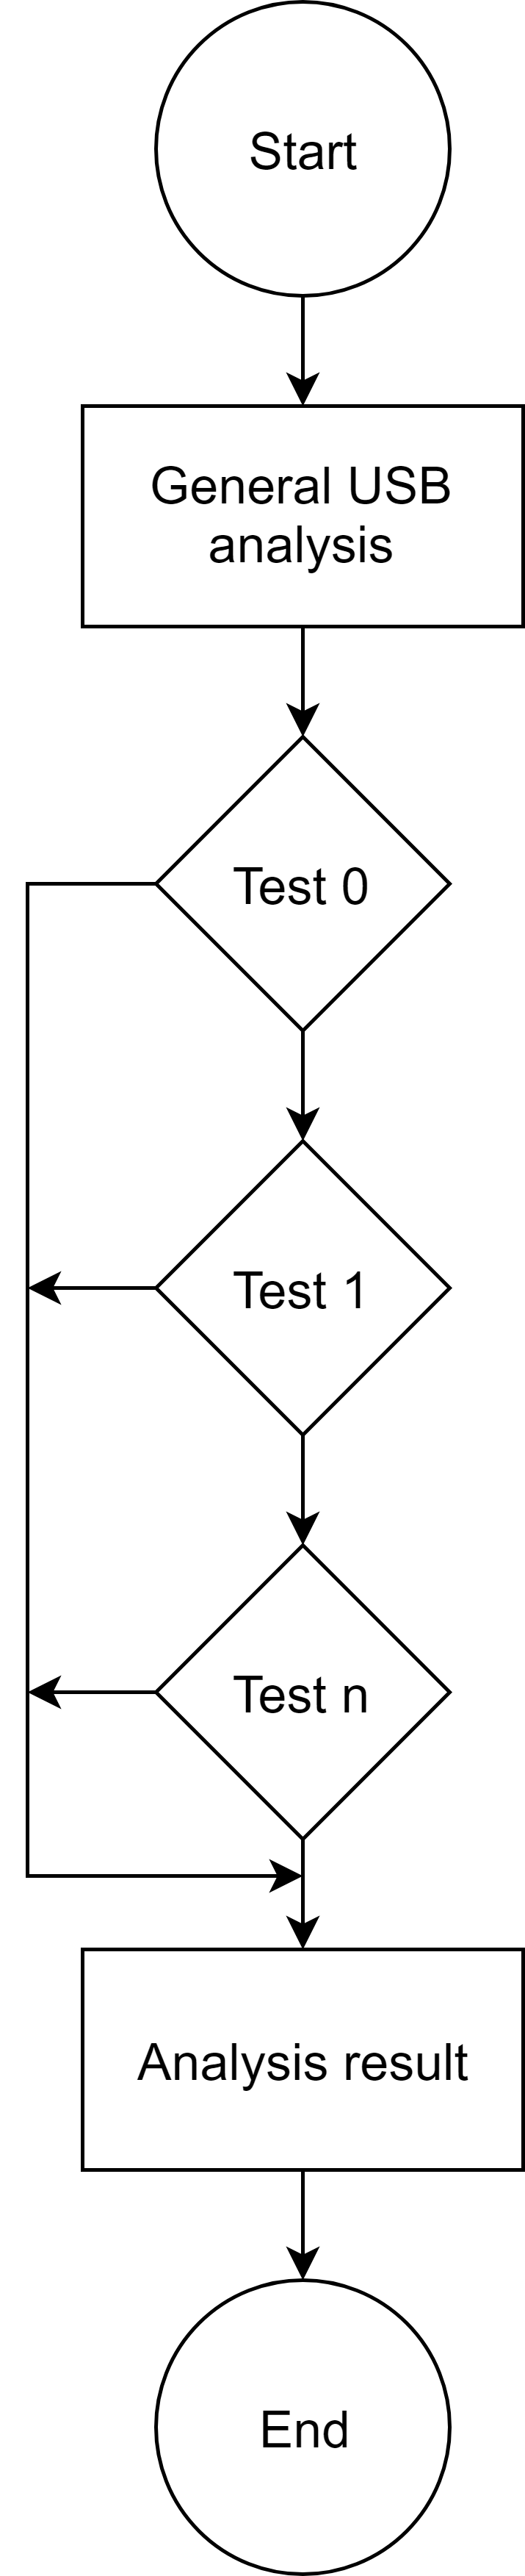
\includegraphics[scale=0.135]{images/tests_flow.png}
    \caption{The diagram shows the way the testing procedure operate. It executes to the $n$th check. If a test is not passed the USB mass storage device will be rendered as dangerous}
    \label{fig:test_flow}
\end{figure}

\subsection{Wiping procedure}
\par \quad After the end of the analyzing process, no matter if the tests were passed or there was an abort, the device wipes all needless files and then reboots. These files include everything that was created for the specific analysis or any other files that are not intended to be on the device. Only files for the testing software and the OS (Operating system) remain.
\par The purpose of this procedure is to make sure that a malware did not create infected files or did not infect temporary ones. After the execution of the procedure the most important files on the device are checked to assure that they are not alternated or infected. The files are being compared to their twins kept on a isolated segment of the memory.

\section{Future development}
\par \quad The current hardware element of the project is aimed for modified Raspberry Pi 3B and Raspberry Pi 4. That is a temporary measure during the early development cycle of Heimdall. Custom designed microprocessor board will be a major part of the future development of the project.Figures \ref{fig:scheme} and \ref{fig:3d_model_concept} shows concept blueprint and 3D model of the board. Another reason to move to a custom board is that it is more modular and can be designed in different ways so it can be commercialized easier.
\par Another major aspect of the future development is deeper research in the USB drivers, self-replicating malwares, firmware alternation and hardware hacking. By alternating the firmware of a USB storage device we can get deeper insight of the bootloading hijacking process and even find new attack vectors.

\begin{figure}[htp]
    \centering
    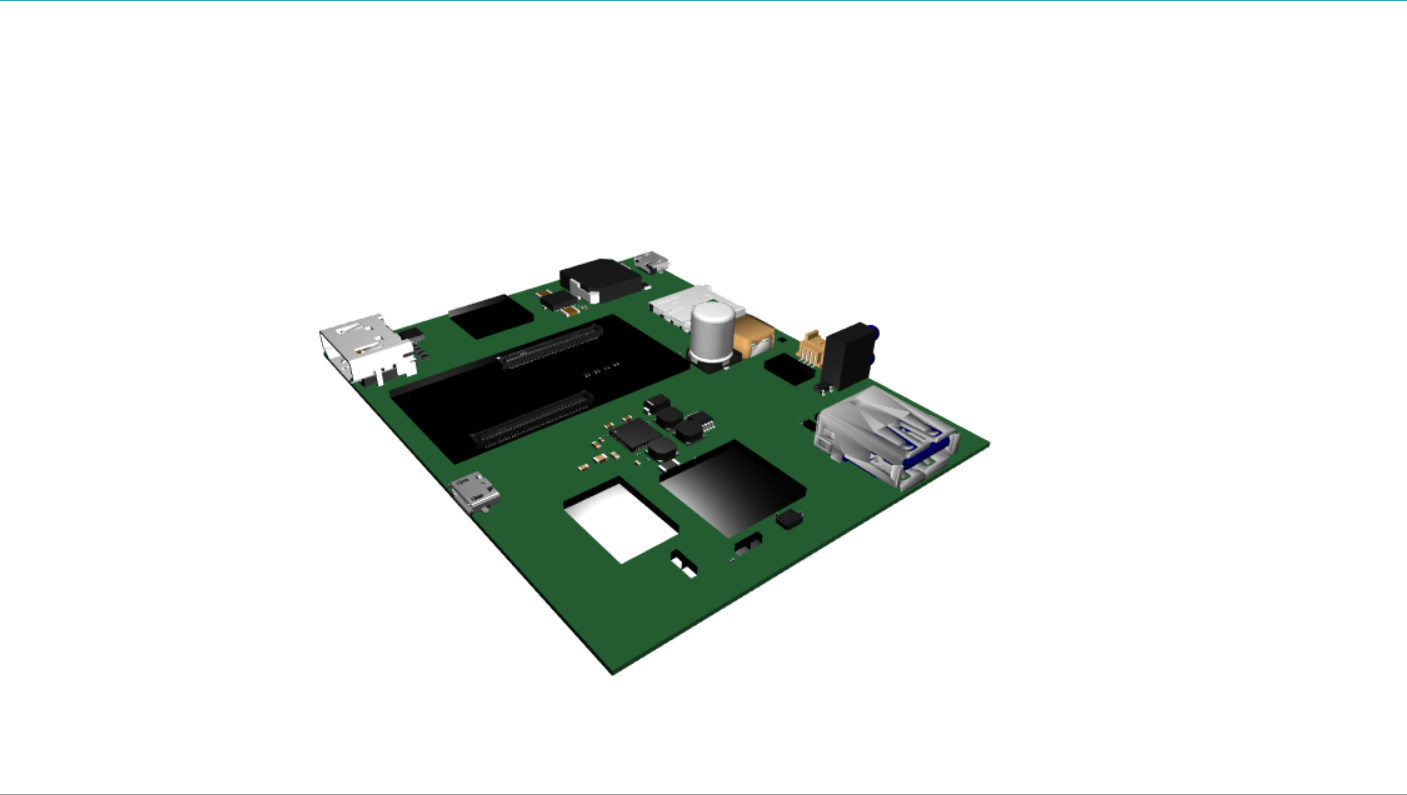
\includegraphics[width=\linewidth]{images/PCB_screenshot.png}
    \caption{A basic 3D model of the concept for custom made microprocessor board.}
    \label{fig:3d_model_concept}
\end{figure}

\begin{figure}[htp]
    \centering
    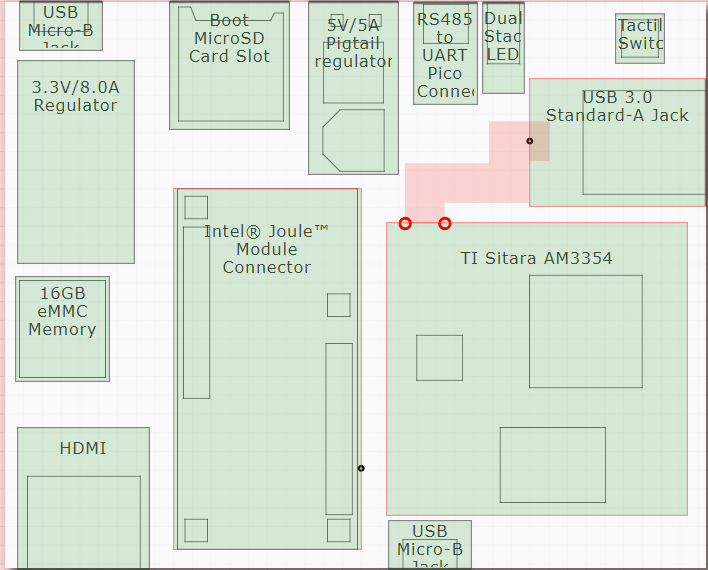
\includegraphics[width=\linewidth]{images/Screenshot_2D.png}
    \caption{The figure shows the blueprint of the 3D model of the microprocessor concept board.}
    \label{fig:scheme}
\end{figure}

\section{Conclusion}
\quad In this paper, we present Heimdall, system of two parts - network isolated embedded system and multiple methods for USB analysis. USB storage devices are constantly used in cyberattacks - from major ones that cause high financial damages to minor ones that can infect your computer with a rootkit. For these reasons USBs are banned or restricted in the enterprise world. To accomplish adequate analysis we use network isolated microprocessor with modified hardware. We can determine if a device has malicious intent through a set of specific tests. If a test is not passed the connected device will be rendered dangerous. We stress that systems like ours must be used in the enterprise world and major infrastructures that use USBs.

\bibliographystyle{plain}
\bibliography{sample-base}

\end{document}
\endinput
